% !TEX root=/home/tavant/these/manuscript/src/manuscript.tex

\section{Monte Carlo computation of the EVDF}
\label{sec-MCM}
  
  The \ac{1D} \ac{PIC} simulations were computed faster than the \ac{2D} simulations, as the latter needed around a week to compute $10\,\micro\second$ on 360 CPUs, while the former needed only a few days on 64 CPUs to compute $20\,\micro\second$ of physical time.
  However, they still take a rather long time, especially when compared to fluid models that can be solved from under one second to around one day on a single core, depending on the hypotheses used.
  
  We have seen that the polytropic index depends on several conditions, as the background pressure (see \cref{fig-p}) but also the densities, sizes, heating mechanism, and so on.
  We have seen in \cref{sec-fluid} that the only value of the polytropic index $\gamma$ is enough to describe the \ac{PIC} simulation.
  As the value of $\gamma$ depends on the \ac{EVDF}, we propose here a Monte Carlo approach that could be used in order to obtain the \ac{EVDF} faster than with a \ac{PIC} simulation.
  A possible application would be similar to \citet{kushner1983}, where the author uses a small population of electrons (typically 300-500) and observes their evolutions in a given plasma potential.
  
  This method gets rid of the Poisson equation, which can take between 30\% and 50\% of the total simulation time.
  Hence, the Debye length does not have to be highly resolved anymore for stability and numerical heating.
  However, we still need to resolve the sheath, which length is of the order of 5 Debye lengths \citep{chabert2014}.
  Consequently, a coarser mesh of cell size 5 times larger can be used.
  The condition on the time step is also reduced.
  This results in a much faster computation.

  \subsection{Description of the Monte Carlo simulation used}

    In order to validate the Monte Carlo approach, we use as reference the converged simulation of the \ac{1D} \ac{PIC} model at a background pressure of $P_n=1$\,mTorr.
    We use the plasma potential $\phi$ computed self-consistently at the end of the \ac{PIC} simulation.
    The Monte Carlo simulation uses the same modules of \LPPic as the \ac{PIC} simulation for the particles, but the fields (charge density, electric field, etc.) are not computed.
    Similarly to the \ac{PIC} simulation, the Monte Carlo simulation is initialized with uniform Maxwellian electrons.
    The electrons motion and collisions are computed as described in \cref{sec-elements}.
    When an electron is collected at the wall, it is re-injected uniformly.

    We validate the Monte Carlo computation by comparing the distribution function obtained with the one measured at the end of the \ac{PIC} simulation.
    \Cref{fig-EEPF_start_end} shows the expected EEPF obtained in the \ac{PIC} simulation with a background pressure of $P=1$\,mTorr.
    The maximum plasma potential, at the center of the domain, is $\max(\phi)=12.2\,\volt$.
    Is also shown in \cref{fig-EEPF_start_end} the EEPF at the beginning of the Monte Carlo computation, which corresponds to the Maxwellian distribution of temperature $\Te=5\,\volt$.
    The results of the Monte Carlo simulation are presented in \cref{subsec-MCMresults}.

    \begin{figure}[!hbt]
      \centering
      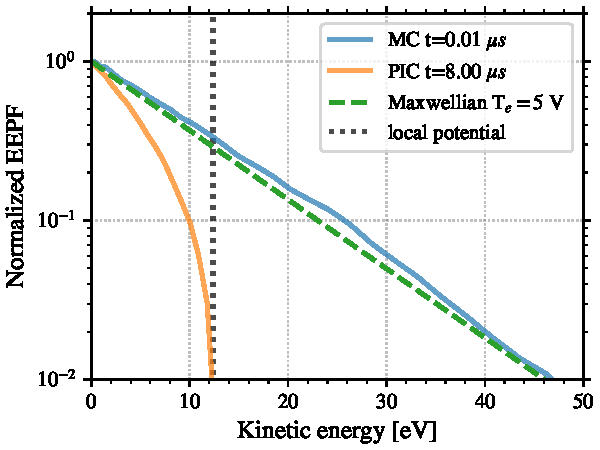
\includegraphics[width=\defaultwidth]{EEPF_PIC.pdf}
      \caption{Electron energy probability function obtained from (orange) the PIC simulation after convergence, and (blue) at the beginning of the Monte Carlo simulation. A Maxwellian distribution function at the $\Te{}_{,inj}$ and the local plasma potential are also given.}
      \label{fig-EEPF_start_end}
    \end{figure}

  \subsection{Results of the Monte Carlo computation} \label{subsec-MCMresults}
    In this section, we describe the temporal evolution of the EEPF in the Monte Carlo (MC) simulation, compared to the EEPF measured in the PIC simulation.
    \paragraph{Beginning of the simulation\\ }
    We start by analyzing the evolution of the EEDF at the very early time of the simulation, from $t=0.01$ to $0.08\,\micro\second$.
    \Cref{fig-zoom_init_Mc} shows the measured electron energy probability function (EEPF) at $3\,\centi\meter$ from the left wall.
    The energy of the electrons is oriented, meaning that the electrons with positive energy are coming from the wall, while the negative energy is used for the electrons going toward the wall.

    \begin{figure}[!hbt]
      \centering
      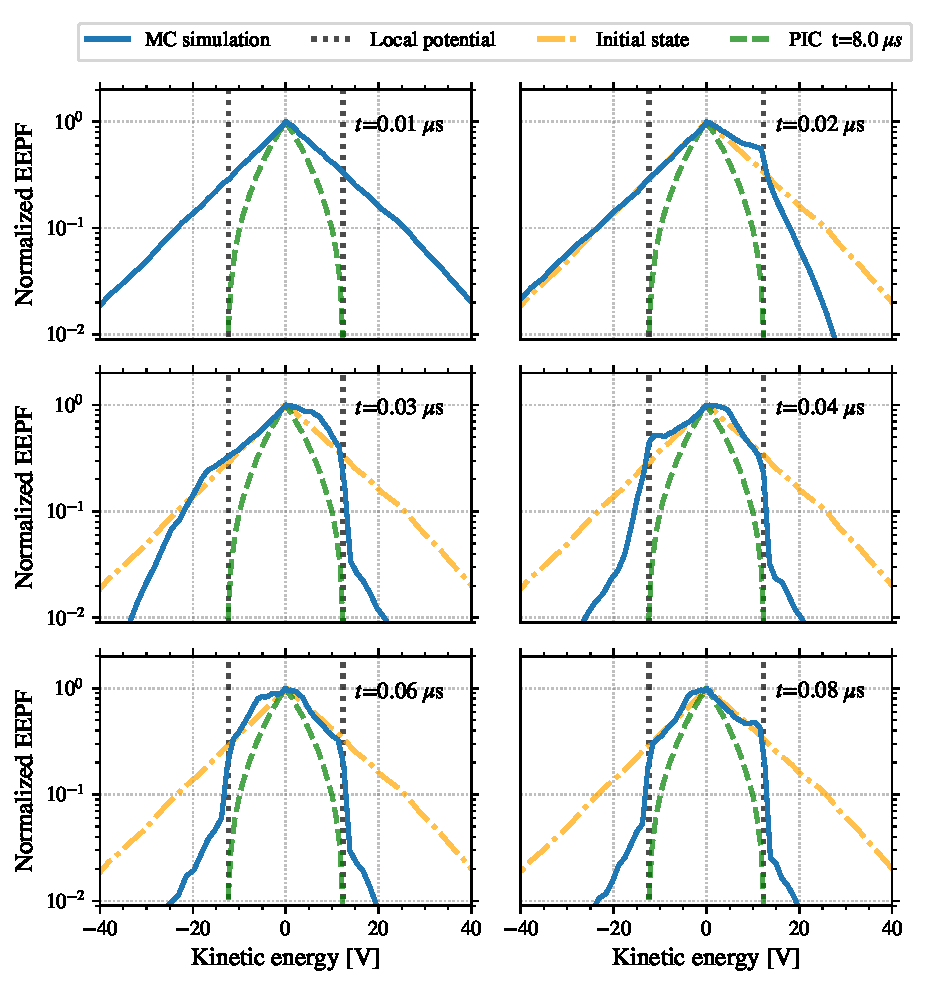
\includegraphics[width=0.9\textwidth]{MC_first_time}
      % \begin{tabular}{@{} cc}
      %   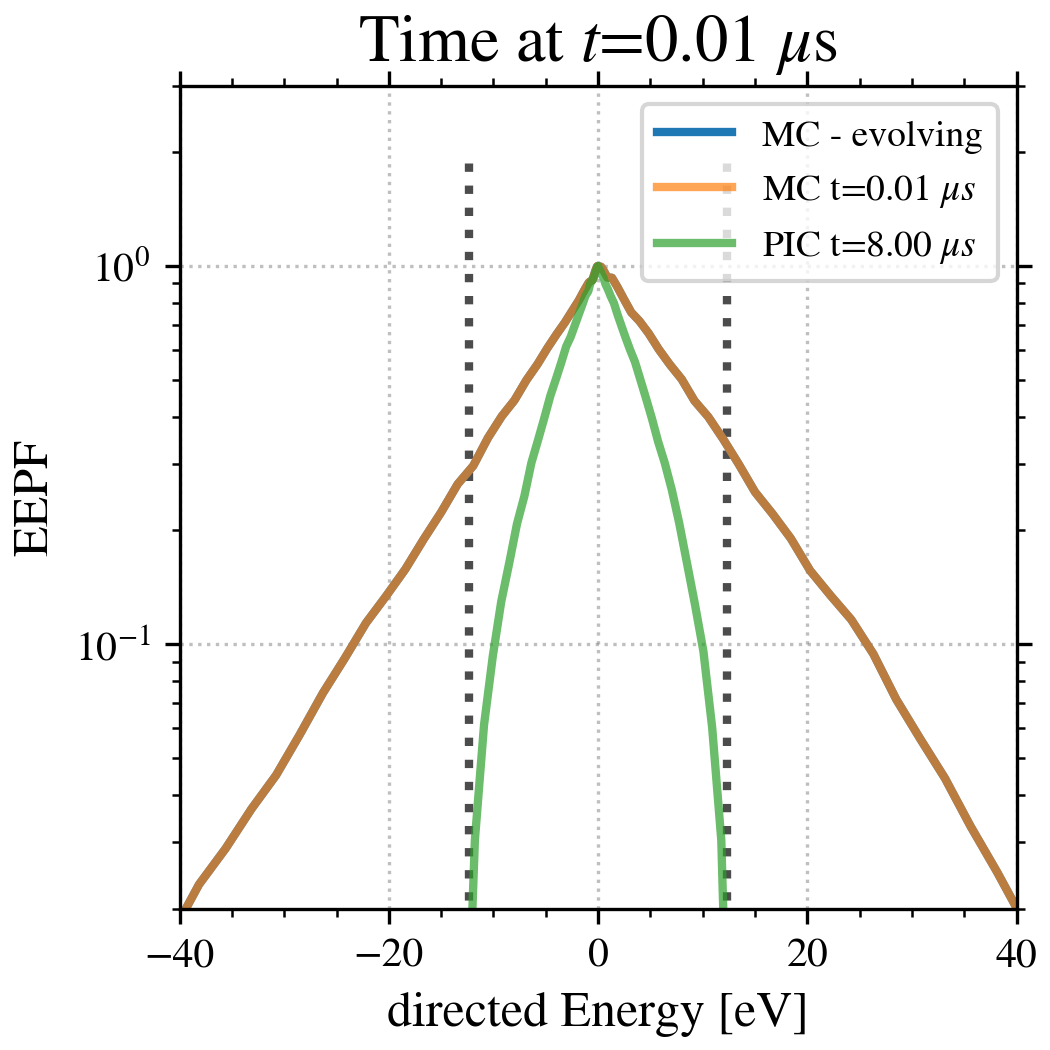
\includegraphics[width=0.4\textwidth]{MCC_EEDF/Heelo_1} &
      %   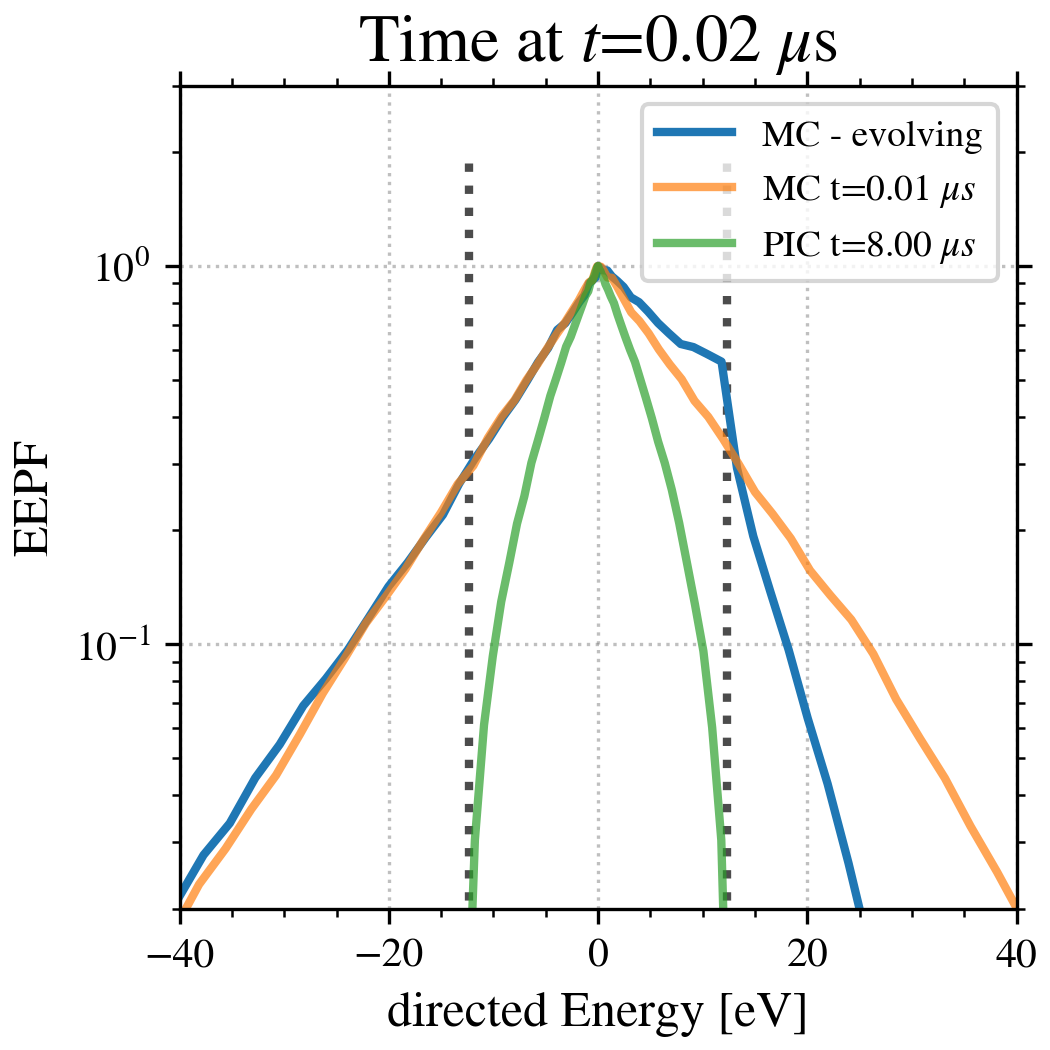
\includegraphics[width=0.4\textwidth]{MCC_EEDF/Heelo_2} \\
      %   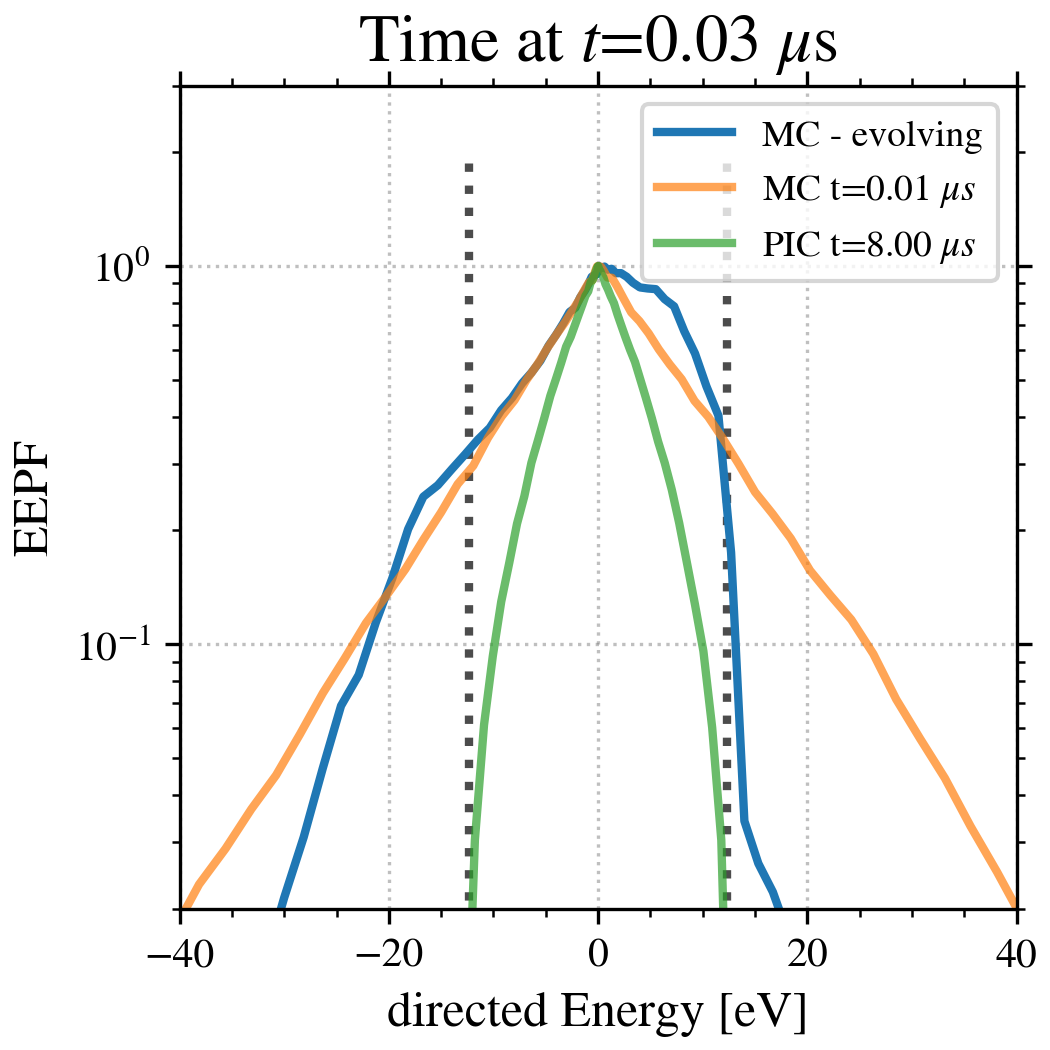
\includegraphics[width=0.4\textwidth]{MCC_EEDF/Heelo_3} &
      %   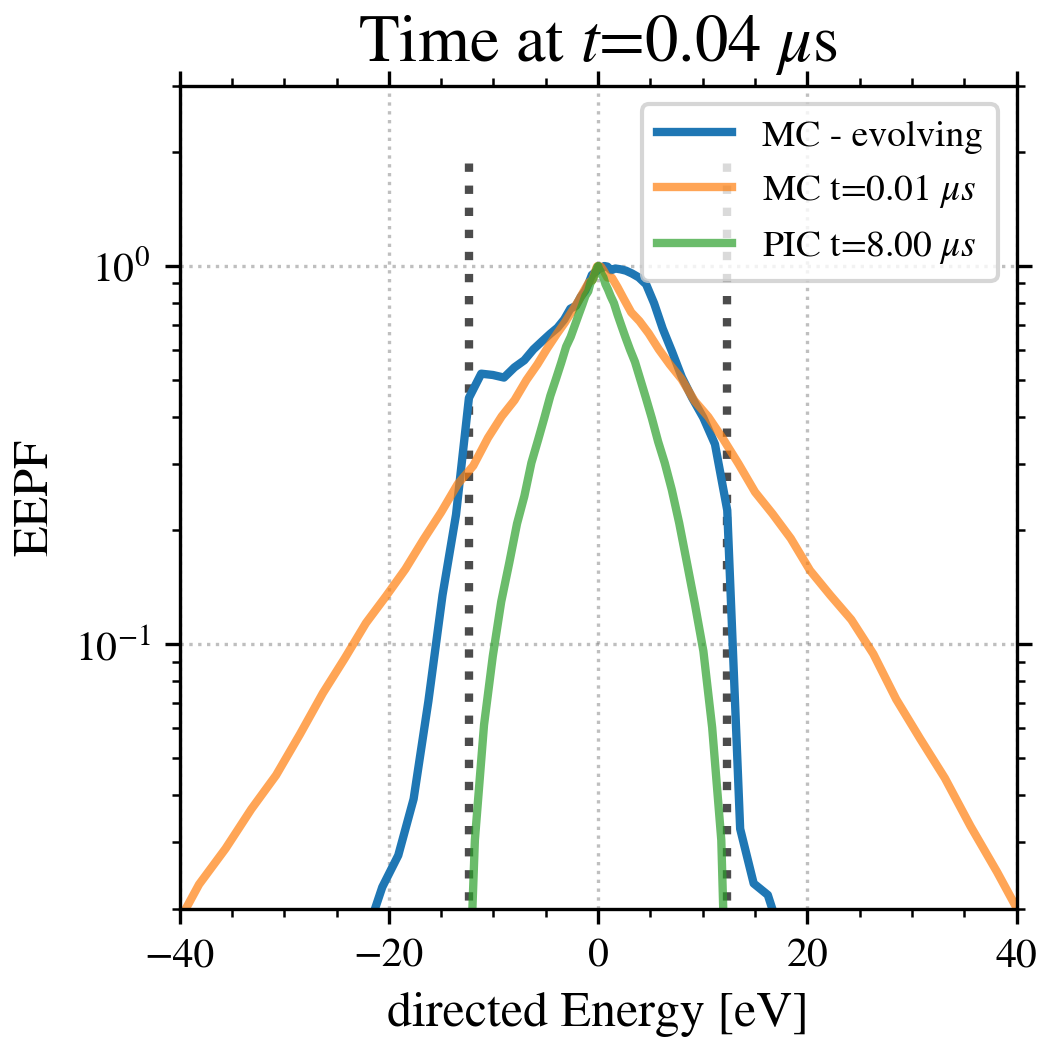
\includegraphics[width=0.4\textwidth]{MCC_EEDF/Heelo_4} \\
      %   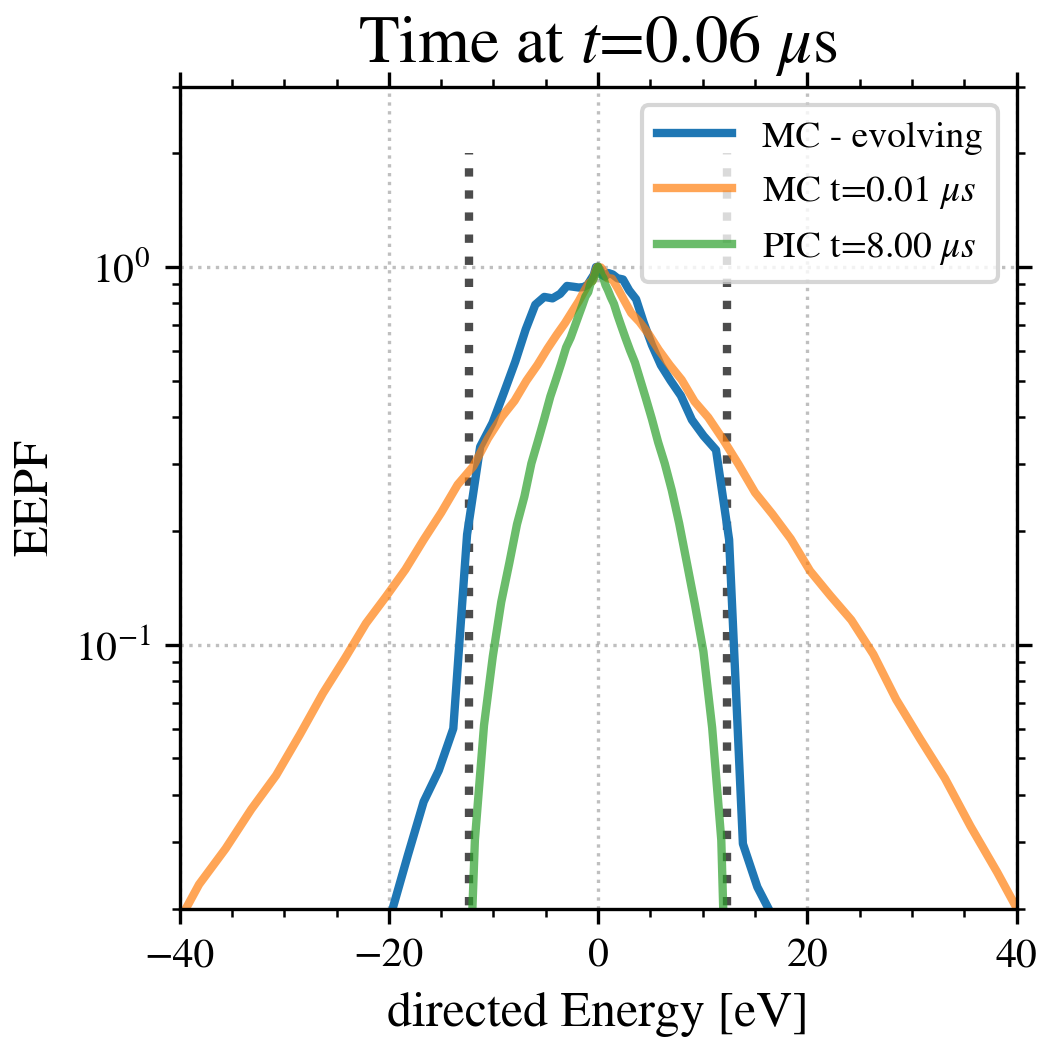
\includegraphics[width=0.4\textwidth]{MCC_EEDF/Heelo_6} &
      %   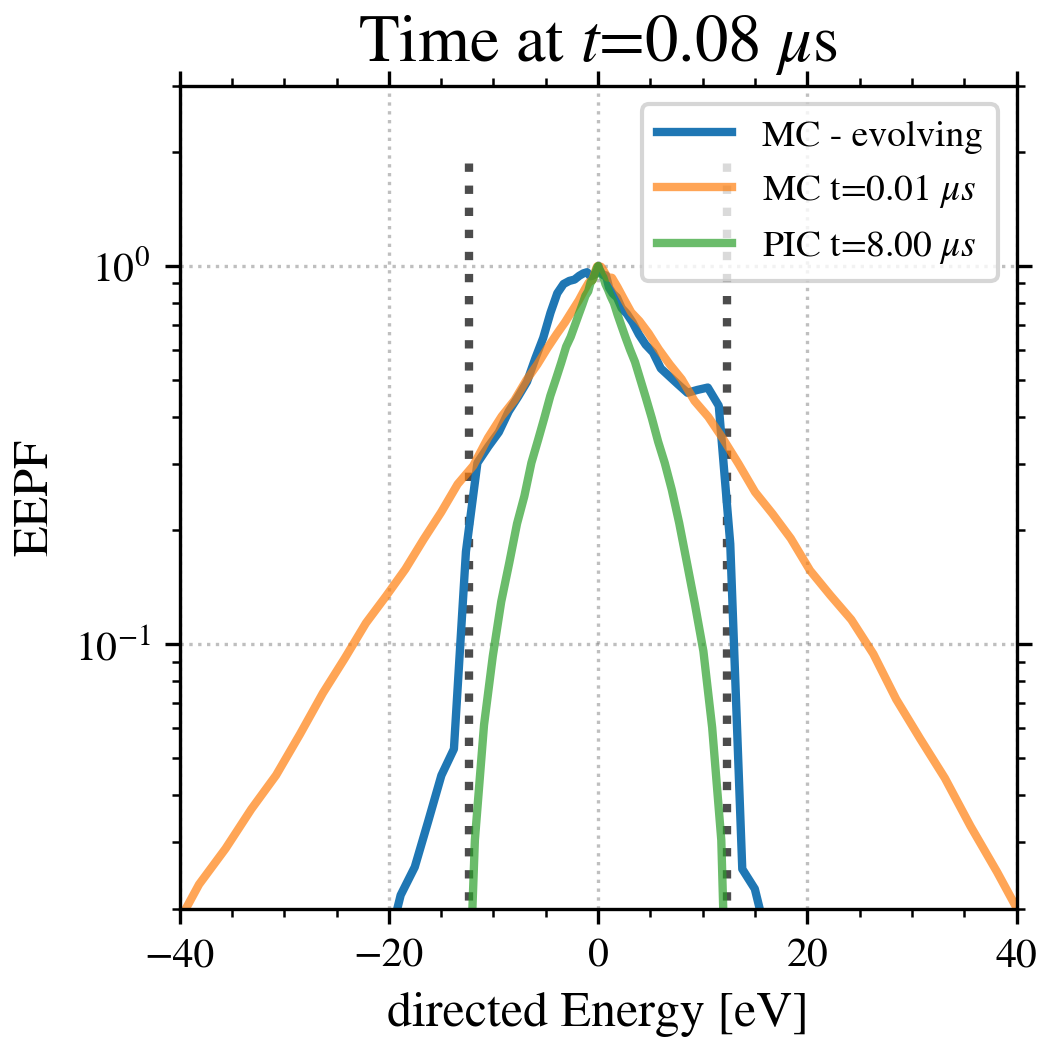
\includegraphics[width=0.4\textwidth]{MCC_EEDF/Heelo_8} \\
      % \end{tabular}
      \caption{Evolution of (blue) the directed EEPF measured at $x=3\,\centi\meter$ from the left wall in the Monte Carlo simulation. The positive energy is used for the electrons going from the wall, while the negative energy represents the electrons moving toward the wall. The dotted lines correspond to the local potential. Are overlaid (dash-dotted orange) the initial Maxwellian distribution (Maxwellian at $\Te=5\,\volt)$ and (dashed green) the EEPF obtained at the end of the \acs{PIC} simulation ($t=8\,\micro\second$). }
      \label{fig-zoom_init_Mc}
    \end{figure}
    

    Two phenomenon can be seen in  \cref{fig-zoom_init_Mc}.
    The first is the rapid decrease of the tail of the distribution function, for energies higher than the plasma potential.
    The tail for positive energy decreases faster than for negative energy, as the EEPF is measured closer to one wall than the other ($x=3\,\centi\meter$ against $L-x=7\,\centi\meter$).
    After $ T \simeq 0.06\,\micro\second$ the two tails are largely depleted, as they are one order of magnitude smaller than the initial Maxwellian EEPF.

    The second phenomena is the presence of waves in the velocity space that can be seen in the low energy populations.
    They are due to the plasma potential profiles.
    Indeed, the electrons are initialized uniformly  with a fixed temperature, hence their total energy depends on the local plasma potential. 

    \paragraph{Convergence of the simulation\\ }

    \Cref{fig-zoom_Mc_later} shows the evolution of the EEDF over a longer time scale from $t=0.1$ to $3.5\,\micro\second$ (compared to $t=0.01$ to $0.08\,\micro\second$ in \cref{fig-zoom_init_Mc}).
    We can see the slow evolution of the low energy population from the initial, but slightly perturbed, Maxwellian distribution toward a distribution of smaller temperature.
    After $t=1.5\,\micro\second$, the EEPF of the Monte Carlo computation is fairly close to -- and converges slowly towards -- the EEPF measured at $t=8\,\micro\second$ in the \ac{PIC} simulation.

    \begin{figure}[!hbt]
      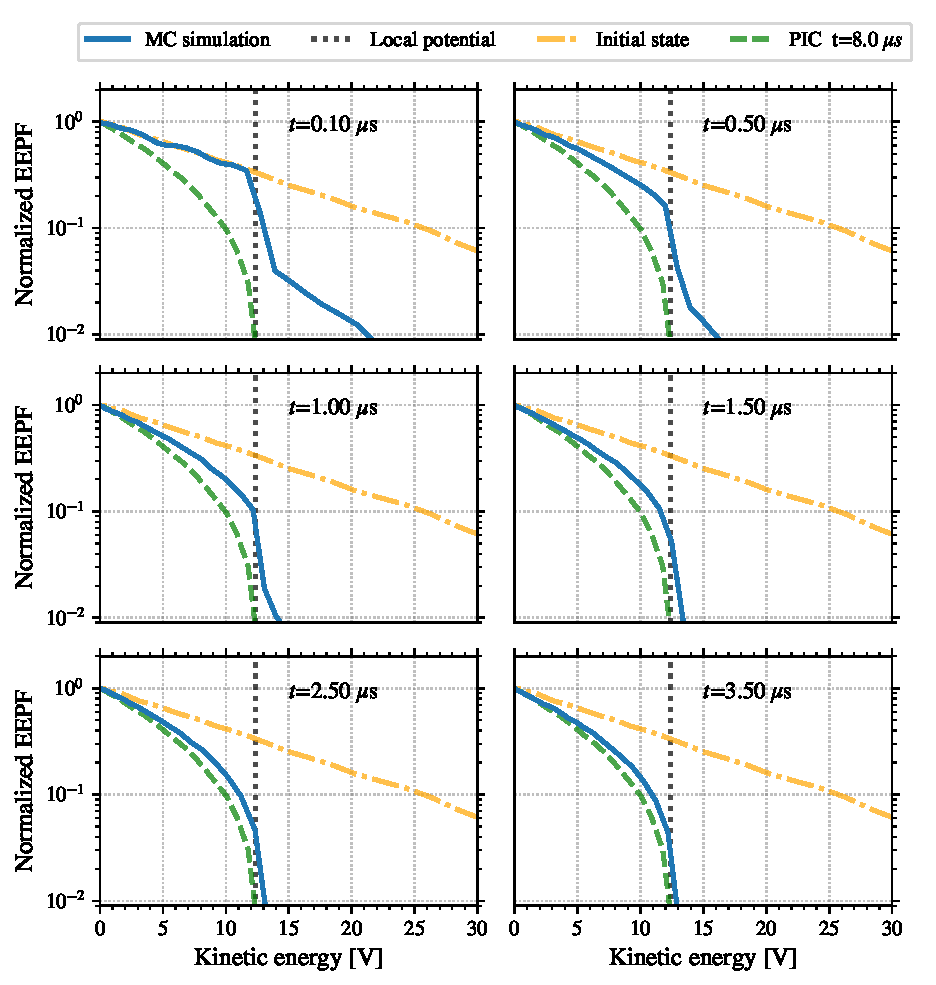
\includegraphics[width=0.9\textwidth]{MC_later_time}

      % \begin{tabular}{@{} ccc}
      %   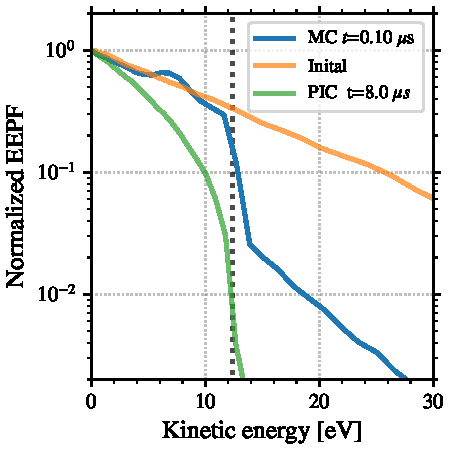
\includegraphics[width=0.3\textwidth]{MCC_EEDF/Heelo_1_10.pdf} &
      %   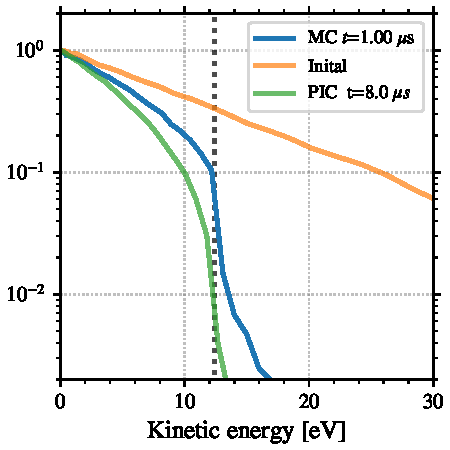
\includegraphics[width=0.3\textwidth]{MCC_EEDF/Heelo_1_100.pdf} &
      %   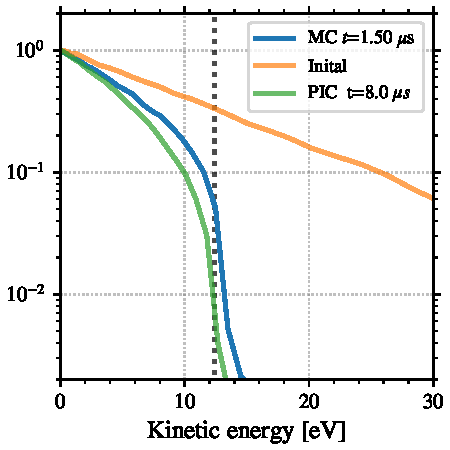
\includegraphics[width=0.3\textwidth]{MCC_EEDF/Heelo_1_150.pdf} \\
      % \end{tabular}
      \caption{Evolution of (blue) the EEPF measured at $x=3\,\centi\meter$ from the left wall in the Monte Carlo simulation. The dotted line corresponds to the local potential. Are overlaid (dash-dotted orange) the initial Maxwellian distribution and (dashed green) the EEPF obtained at the end of the \acs{PIC} simulation ($t=8\,\micro\second$). }
      \label{fig-zoom_Mc_later}
    \end{figure}

    \vspace{1em}
    This Monte Carlo investigation has shown that in the \ac{1D} model at $P_n=1$\,mTorr, the EEPF depends on the absorption at the wall but also on the electron-neutral collisions.
    The final shape of the distribution is not simple, and is difficult to describe and predict analytically.
    However, given the profile of the plasma potential, the Monte Carlo computation reproduces the same distribution in a much shorter time compared to the \ac{PIC} simulation. 
    The obtained EEPF can then be used to determine the electron density and temperature evolution in a low pressure plasma where electrons are non-local.
    This could be used to determine efficiently, and precisely, the electron polytropic coefficient to use in a fluid model.

  \subsection{Discussion on the different time scales}
    The results presented in the previous section show two main time scales.
    In this section, we compare the observed time scales with the theoretical times.
    The electrons collected at the wall have a kinetic energy at least equal to the potential drop to the wall $\ek = e \dphi$, which corresponds in our case to a limit velocity of $v_{\rm lim} = \sn{1.5}{6} \,\meter\per\second$.
    Hence, the limit time of flight between the two boundaries is
    \[ T_{\rm flight} = \frac{L}{v_{\rm lim}} = 0.068 \,\micro\second.  \]
    This is in agreement with the results of \cref{fig-zoom_init_Mc}, where we see that the high energy tails are depleted around $t=0.06\,\micro\second$.
    
    \vspace{1em}
    The electron-neutral scattering frequency is computed for a background pressure of $0.13$\,Pa (${1}$\,mTorr) at the temperature of $300\,\kelvin$, which corresponds to a neutral density of $${n_g = \sn{3.2}{19} \meter^{-3}}.$$
    For an electron temperature of $5\,\volt$, the thermal electron-neutral elastic scattering frequency for argon is \citep[p.73]{lieberman2005}
    \[ \nu_{\rm ela} = 4.70 \,\mega\hertz,  \] 
    which corresponds to a period of $\tau_{\rm ela} = 0.2 \,\micro\second$.
    This period is shorter than the one observed in the Monte-Carlo simulation, as we see in \cref{fig-zoom_Mc_later} that the low energy part of the EEPF is significantly affected after $t=1\,\micro\second$.
    
    This discrepancy can be due to two reasons.
    First, at high energy the electron-neutral scattering is not isotropic, but instead gives mostly small angles (forward scattering) \citep{vahedi1995}.
    Hence, a large number of collisions is required for the isotropization to be observable.
    Secondly, the argon presents a significant Ramsauer minimum (a quantum mechanical resonance \citep{lieberman2005}) at $0.3 \,\volt$, were the cross-section is two orders of magnitude lower than at $5\,\volt$.  
    
        \paragraph{Numerical artifacts \\}
        In PIC simulations, numerical parameters can induce numerical heating and thermalization \citep{lai2014}.
        The numerical heating has been studied in detail \citep{birdsall1991}.
        It is due to aliasing effects, and depends on the grid size, time step and number of particles per cell.
        It is important to carefully choose these parameters to reduce the effect of the heating.

        The thermalization is the fact that the distribution of the particle tends toward a Maxwellian.
        It originates from fluctuations of the electric field due to the discretization of the particles.
        The first studies showed that the thermalization time $\tau_T$ depends on $N_D$ the number of (numerical) particles per Debye sphere \citep{dawson1964,montgomery1970}.
        The presence of collisions can affect $\tau_T$  \citep{turner2006,lai2014}.
        In \citet{turner2006}, the author observed the evolution of the thermalization time with $N_D$ as
        \begin{equation} \label{eq-taut}
          \tau_T = \frac{1}{\omega_{pe}} \frac{34.4}{N_D^{-2} + 28.0 N_D^{-1} \frac{\nu_m}{\omega_{pe}}}
        \end{equation}
        which gives in our condition a time-scale several orders of magnitude larger than the typical simulation time.
        We confirmed it by doubling the number of particle per cell for one pressure condition, and no observable impact has been detected.
        Hence, the effects of numerical parameters on the simulation results are expected to be negligible.
